\usepackage[T1]{fontenc} % Codificación de las fuentes utilizadas
\usepackage[spanish]{babel} % Español como idioma principal del texto (permite hyphenation de palabras al final de una línea)


\usepackage{graphicx}
\usepackage{url}

\graphicspath{{Figures/}{Diagrams}{Chapters/}}  % Location of the graphics files (set up for graphics to be in PDF format)

\selectlanguage{spanish}

\setcounter{tocdepth}{1}

% Include any extra LaTeX packages required
\usepackage[square, numbers, comma, sort&compress]{natbib}  % Use the "Natbib" style for the references in the Bibliography
\usepackage{verbatim}  % Needed for the "comment" environment to make LaTeX comments
\usepackage{vector}  % Allows "\bvec{}" and "\buvec{}" for "blackboard" style bold vectors in maths
\hypersetup{urlcolor=blue, colorlinks=true}  % Colours hyperlinks in blue, but this can be distracting if there are many links.
\usepackage{hyperref}
% \usepackage[pdfauthor={Diego Martín Arroyo},
%             pdftitle={Diseño e implementación de un sistema de computación distribuida con
% Raspberry Pi, y estudio comparativo del mismo frente a otras soluciones},
%             pdfsubject={Memora del Trabajo de Fin de Grado},
%             pdfproducer={XeLaTeX with hyperref},
%             pdfcreator={XeLaTeX},
%             pdfkeywords={Computación Paralela, Sistema Distribuido, Raspberry}
%             ]{hyperref}
%% ----------------------------------------------------------------

%% --------------------------------------------------------------------------------------------------------------------------------
%http://tex.stackexchange.com/a/85218/76599
\usepackage{fancyvrb}
\usepackage[dvipsnames]{xcolor}

% redefine \VerbatimInput
\RecustomVerbatimCommand{\VerbatimInput}{VerbatimInput}% Inclusión de archivos de texto plano
{fontsize=\footnotesize,
 %
 frame=lines,  % top and bottom rule only
 framesep=2em, % separation between frame and text
 rulecolor=\color{Gray},
 %
 label=\fbox{\color{Black}data.txt},
 labelposition=topline,
 %
 commandchars=\|\(\), % escape character and argument delimiters for
                      % commands within the verbatim
 commentchar=*        % comment character
}

\usepackage{listings} % Requerido para la inserción de código
%Listings command

\usepackage{float}
\newcommand*\lstinputpath[1]{\lstset{inputpath=#1}}
\lstinputpath{Code/}

\newcounter{undefinedreferences}
\setcounter{undefinedreferences}{0}

\newcommand{\citationneeded}[1][None]{\stepcounter{undefinedreferences}\textsuperscript{\color{blue} [Citation needed: #1]}}

\newcommand{\checkreferences}{
\ifnum\value{undefinedreferences} > 0
\begin{center}
\immediate\write18{wget -O Figures/protester.png -nc http://imgs.xkcd.com/comics/wikipedian_protester.png}
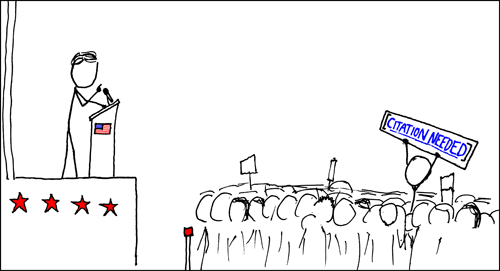
\includegraphics[width=\textwidth]{protester.png}\\
There are \arabic{undefinedreferences} undefined references
\end{center}
\else
No undefined references. Good!
\fi
}


%https://github.com/pads-fhs/LaTeX-Template-Thesis/blob/master/lststyles.tex
\lstdefinelanguage{JavaScript}{
  keywords={typeof, new, true, false, catch,%
    function, return, null, catch, switch, var,%
    if, in, while, do, else, case, break},
  ndkeywords={class, export, boolean, throw, implements, import, this},
  sensitive=false,
  comment=[l]{//},
  morecomment=[s]{/*}{*/},
  morestring=[b]',
  morestring=[b]"
}
\newcommand{\lstsetjavascript}{
  \lstset{
		language=JavaScript,
		breaklines=true,
		commentstyle=\textit,
		basicstyle=\ttfamily,
		keywordstyle=\bfseries,
		stringstyle=\ttfamily,
		showstringspaces=false,
		frame=single,
		tabsize=2
  }
}

\lstdefinelanguage{log}{
  keywords={typeof, new, true, false, catch,%
    function, return, null, catch, switch, var,%
    if, in, while, do, else, case, break},
  ndkeywords={class, export, boolean, throw, implements, import, this},
  sensitive=false,
  comment=[l]{//},
  morecomment=[s]{/*}{*/},
  morestring=[b]',
  morestring=[b]"
}
\newcommand{\lstsetlog}{
  \lstset{
		language=log,
		breaklines=true,
		commentstyle=\textit,
		basicstyle=\ttfamily,
		keywordstyle=\bfseries,
		stringstyle=\ttfamily,
		showstringspaces=false,
		frame=single,
		tabsize=2
  }
}

\lstloadlanguages{Java,XML, JavaScript, log}

\newcommand{\javascriptcode}[4]{
	\lstinputlisting[caption=#2,label=#1, firstline=#3, lastline=#4]{#1.json}
}

\newcommand{\logcode}[4]{
	\lstinputlisting[caption=#2,label=#1, firstline=#3, lastline=#4]{#1.log}
}

\usepackage[bottom]{footmisc} %The footnotes go at the bottom of t\usepackage{dtklogos}he page, instead next to the last line.
%Ajustes para Java
% \lstset{
% 	language=java,
%  	frame=single, % Un marco simple alrededor del código
%     basicstyle=\small\ttfamily, % Utilizar fuente true type pequeña
%     keywordstyle=[1]\color{Blue}\bf, % Funciones en negrita y azul
%     keywordstyle=[2]\color{Purple}, % Argumentos en morado
%     keywordstyle=[3]\color{Blue}\underbar, % Funciones personalizadas subrayadas en azul
%     identifierstyle=, % Nada especial acerca de identificadores
%     commentstyle=\usefont{T1}{pcr}{m}{sl}\color{Green}\small, % Los comentarios se renderizan en fuente pequeña verde
%     stringstyle=\color{Purple}, % Cadenas en morado
%     showstringspaces=false, % No se muestran los espacios entre cadenas
%     tabsize=5, % 5 espacios por tabulado
%     %
%     % Put standard Perl functions not included in the default language here
%     %morekeywords={rand},
%     %
%     % Put Perl function parameters here
%     %morekeywords=[2]{on, off, interp},
%     %
%     % Put user defined functions here
%     %morekeywords=[3]{test},\usepackage{dtklogos}
%    	%
%     morecomment=[l][\color{Blue}]{...}, % Line continuation (...) like blue comment
%     numbers=left, % Número de línea a la izquierda
%     firstnumber=1, % Número de línea comienza en 1
%     numberstyle=\tiny\color{Blue}, % Los números de línea son azules y pequeños
%     stepnumber=5, % Los números de línea van de 5 en 5
%     breaklines=true % Salto de línea si el texto no entra. See http://stackoverflow.com/a/1875803
% }

%\usepackage{xltxtra} % XeLaTeX logo. Yep, just that
%http://tex.stackexchange.com/a/73179/76599
\usepackage{metalogo}
%\usepackage{dtklogos} %BibTeX logo
\def\BibTeX{{\rm B\kern-.05em{\sc i\kern-.025em b}\kern-.08em
    T\kern-.1667em\lower.7ex\hbox{E}\kern-.125emX}}

\newenvironment{alignedDescription}[2][0pt]
  {\begin{list}{}%
    {\renewcommand\makelabel[1]{\textsf{\textbf{##1}}\hfil}%
     \settowidth\labelwidth{\makelabel{#2}}%
     \setlength\leftmargin{\labelwidth+\labelsep + #1}}}%
  {\end{list}}

\newenvironment{elements}
{\begin{quote}\itshape\centering\small}
{\end{quote}}

\newenvironment{cabstract}
{\begin{quote}\itshape\centering\small}
{\end{quote}}

%\usepackage[xindy]{glossaries}
%\newcommand{\chapterabstract}{1}{
%	\begin{center}
%	\small\textit
%	#1
%	\end{center}
%}

\usepackage{xcolor,colortbl}
\usepackage{xcolor}
\usepackage{pdfpages}
\hypersetup{
    colorlinks,
    linkcolor={red!50!black},
    citecolor={blue!50!black},
    urlcolor={blue!80!black}
}

\newcommand{\hmwkTitle}{Gestión del proyecto} % Assignment title
\newcommand{\hmwkDueDate}{Miércoles,\ 8\ de\ julio\ de\ 2015}
\newcommand{\hmwkClassInstructor}{Rodrigo Santamaría} % Teacher/lecturer
\newcommand{\hmwkAuthorName}{Diego Martín Arroyo} % Your name
\newcommand{\hmwkSubject}{6} % Evaluation subject number

%----------------------------------------------------------------------------------------
%   TITLE PAGE
%----------------------------------------------------------------------------------------
\newcommand{\ordinalindicator}{\hspace{-1.5mm}$\phantom{a}^{\circ}$}
\title{\hmwkTitle}
\author{\textbf{\hmwkAuthorName}}
\date{\hmwkDueDate}
\begin{document}
\maketitle

\tableofcontents

\section{Introducción}

El presente documento tiene como objetivo describir todos los aspectos relativos a la gestión del proyecto no detallados en la memoria principal del mismo, definiendo las secciones del mismo siguiendo las indicaciones del \textit{Project Management Body of Knowledge} (\textbf{PMBOK}).

\section{Planificación}

Uno de los aspectos fundamentales a la hora de realizar cualquier proyecto de desarrollo de una envergadura considerable es la planificación del mismo. Esta necesidad es mayor acuciante cuando se consideran diferentes restricciones como las dadas en el presente proyecto, generalmente de carácter temporal. Otro aspecto a considerar en este proyecto a la hora de elegir la metodología a utilizar es la falta de experiencia con el tipo de \textit{software} a desarrollar. La incertidumbre es muy alta, y por tanto es crucial elegir una dinámica de desarrollo tolerante a cambios inesperados y ``caminos sin salida''.

La metodología por tanto debe ser elegida cuidadosamente, basándose en modelos probados y conocidos, adaptando si es necesario estos a las necesidades específicas del proyecto.

\subsection{Definición de la metodología}

Tras varias reuniones en las que se establecen los objetivos globales del proyecto, realizadas en septiembre de 2014 y a partir de febrero de 2015 de forma más intensiva, se decide en marzo, previamente a que comience de forma intensiva el desarrollo del proyecto el uso de una metodología ágil. Esta se basará en la realización de etapas de trabajo de corta duración (entre una y dos semanas). Con reuniones de equipo entre cada una de ellas. En estas reuniones se evalúan los resultados, identifican situaciones críticas y se definen los objetivos de la siguiente etapa.

A fin de dotar al proyecto de la flexibilidad necesaria para subsanar la falta de experiencia en diferentes componentes del proyecto, se opta por basar los diferentes desarrollos en un proceso orientado a prototipos incrementales, productos \textit{software} incompletos que incorporan diferentes partes de la funcionalidad a desarrollar y que son evaluables. De esta forma, es posible validar la viabilidad de un producto sin que el mismo esté completo, realizar un análisis de alternativas detallado (elaborando prototipos orientativos en poco tiempo) del mismo y añadir nuevas mejoras de forma incremental (de esta forma, en caso de que no todos los objetivos marcados puedan marcarse, el resto del producto será funcional).

Esta metodología ha permitido la ampliación de los objetivos del proyecto sin alterar el ritmo de desarrollo. El desarrollo de herramientas como \textbf{MarcoPolo}, hoy parte crucial del sistema e inicialmente no planteada, ha sido factible gracias a la elección de este proceso.

En cada una de las iteraciones se llevan a cabo las actividades de iniciación, planificación, ejecución, control y conclusión habituales en todo proyecto.

\subsubsection{Herramientas de planificación}

Se considera que el uso de una herramienta para la gestión del proyecto es beneficiosa. Su utilización facilita la identificación de tareas a realizar, coordinar el equipo y obtener de forma sencilla una visualización del estado del proyecto.

Se valoran varias herramientas con las que se cuenta experiencia o conocidas. \textbf{Microsoft Project}\footnote{\href{https://products.office.com/es-ES/project}{https://products.office.com/es-ES/project}}, \textbf{JIRA}\footnote{\href{https://www.atlassian.com/software/jira}{https://www.atlassian.com/software/jira}} y \textbf{Redmine}\footnote{\href{http://redmine.org/}{http://redmine.org/}}. Microsoft Project es descartado por la falta de funcionalidad en línea (a menos que se utilice Microsoft Project Server, cuya adquisición no es considerada. El hecho de contar con una instancia en línea permite coordinar un equipo que no se encuentra en la misma localización física y el acceso a la plataforma desde cualquier dispositivo (gran parte de la planificación se ha realizado a través de un cliente móvil para la plataforma Android). En el caso particular de este proyecto, como Trabajo de Fin de Grado, el uso de este tipo de instancia permite a los tutores contar con un seguimiento del alumno sin la necesidad de reuniones y a los evaluadores del mismo la revisión de la gestión del proyecto de forma sencilla.

\textbf{JIRA} es descartado al no contar con experiencia de uso y su coste, previsiblemente alto (así como los costes de alojamiento). \textbf{Redmine} es una herramienta libre y gratuita, con la que se cuenta experiencia, satisface todas las demandas planteadas y su consumo es pequeño. Es por ello que es la alternativa a utilizar en el proyecto.

Redmine define todas las tareas del proyecto en ``asuntos'' \textit{issues}, que pueden ser de tres tipos: (error (\textit{bug}), funcionalidad (\textit{feature}) o soporte (\textit{support}). Estos asuntos pueden ser marcados temporalmente, incluyendo estimaciones de tiempo, progreso, notas y comentarios. Todos los datos introducidos a la plataforma serán representados en un diagrama de Gantt que representará el estado de desarrollo del proyecto.

La instancia de Redmine utilizada se encuentra alojada en \href{http://redmine.martinarroyo.net/}{http://redmine.martinarroyo.net/}. El acceso a la misma no requiere autenticación.

\begin{figure}[H]
	\centering
	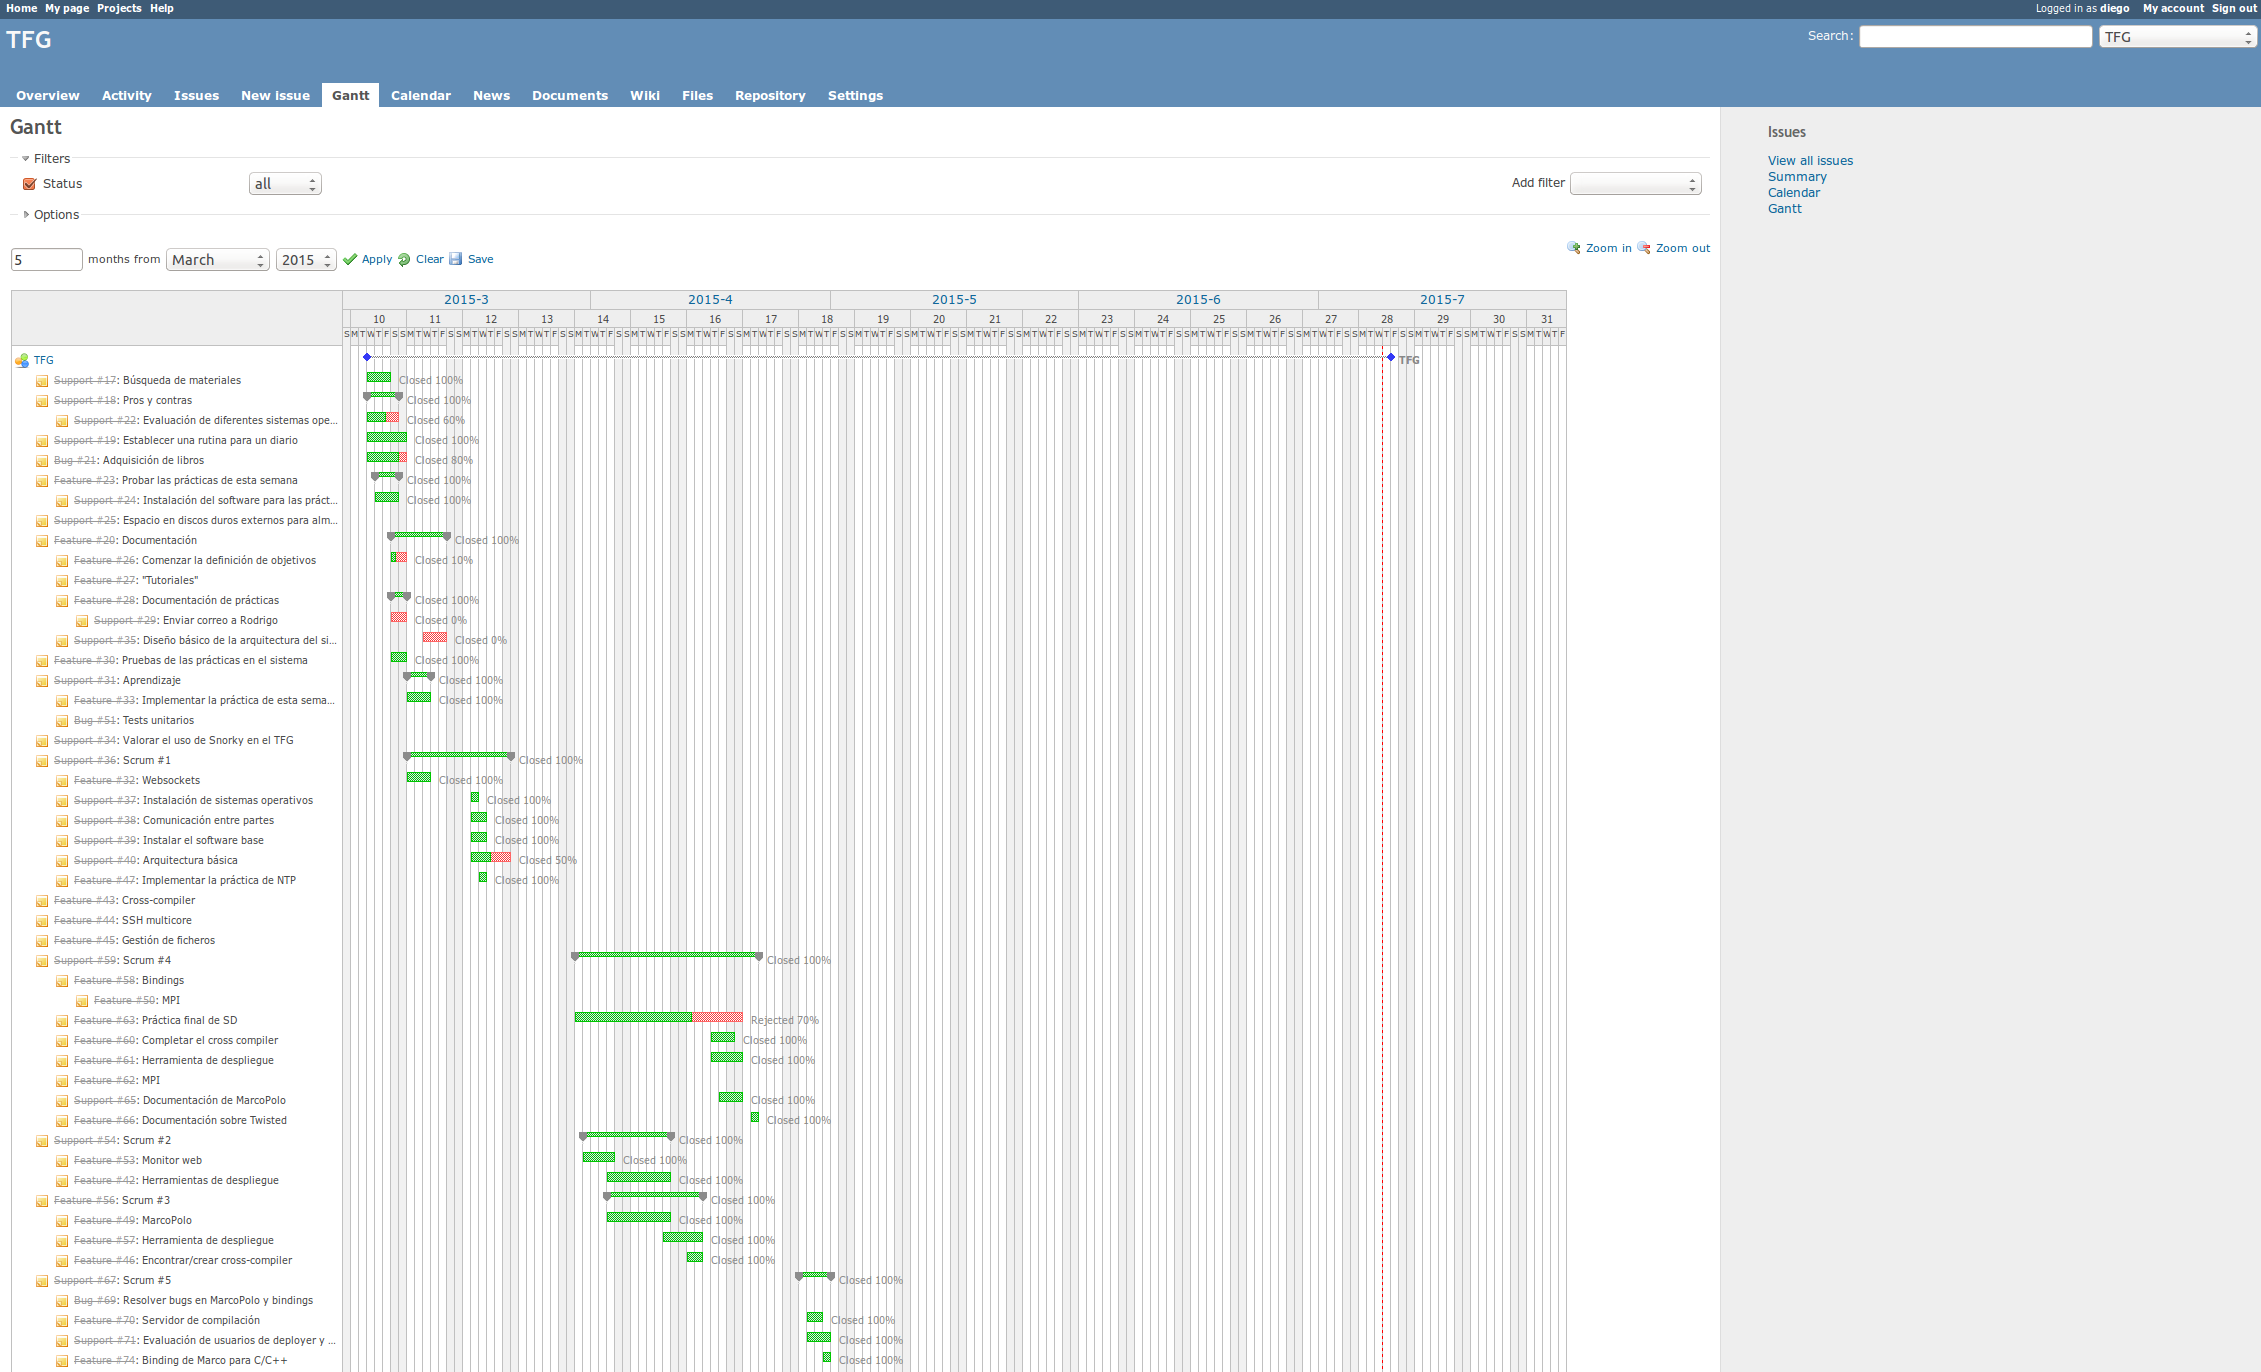
\includegraphics[width=0.9\textwidth]{Figures/redminevista}
	\caption{Vista parcial de todos los asuntos del proyecto en Redmine}
\end{figure}


\subsubsection{Planificación temporal}

En total se han realizado un total de 13 iteraciones en un periodo de 16 semanas, marcadas por reuniones de inicio y fin en cada una de ellas. A continuación se detalla brevemente las características de cada una de ellas:

\paragraph{Iteración 1\\}
\begin{itemize}
\item \textbf{Fecha de inicio}: 09/03/2015
\item \textbf{Fecha de fin}: 21/03/2015
\item En esta iteración comienza formalmente el desarrollo del proyecto.
\item \textbf{URL}: \href{http://redmine.martinarroyo.net/issues/36}{http://redmine.martinarroyo.net/issues/36}
\end{itemize}


\paragraph{Iteración 2\\}
\begin{itemize}
\item \textbf{Fecha de inicio}: 31/03/2015
\item \textbf{Fecha de fin}: 10/04/2015
\item Los esfuerzos se concentran en las herramientas de despliegue y el monitor web.
\item \textbf{URL}: \href{http://redmine.martinarroyo.net/issues/54}{http://redmine.martinarroyo.net/issues/54}
\end{itemize}

\paragraph{Iteración 3\\}
\begin{itemize}
\item \textbf{Fecha de inicio}: 03/04/2015
\item \textbf{Fecha de fin}: 14/04/2015
\item Comienza el desarrollo del protocolo de descubrimiento de servicios \textbf{MarcoPolo}, la creación de un compilador cruzado y la herramienta de despliegue. Esta iteración continúa el trabajo llevado a cabo en la iteración 2.
\item \textbf{URL}: \href{http://redmine.martinarroyo.net/issues/56}{http://redmine.martinarroyo.net/issues/56}
\end{itemize}


\paragraph{Iteración 4\\}
\begin{itemize}
\item \textbf{Fecha de inicio}: 30/03/2015
\item \textbf{Fecha de fin}: 21/04/2015
\item Comienza el desarrollo de los \textit{Bindings} de \textbf{MarcoPolo}, se define el compilador cruzado y MPI es incluido en el proyecto
\item \textbf{URL}: \href{http://redmine.martinarroyo.net/issues/59}{http://redmine.martinarroyo.net/issues/59}
\end{itemize}


\paragraph{Iteración 5\\}
\begin{itemize}
\item \textbf{Fecha de inicio}: 27/04/2015
\item \textbf{Fecha de fin}: 30/04/2015
\item Se establece un servidor de compilación y la expansión del número de bindings comienza, así como diferentes procesos de evaluación de usuarios.
\item \textbf{URL}: \href{http://redmine.martinarroyo.net/issues/67}{http://redmine.martinarroyo.net/issues/67}
\end{itemize}


\paragraph{Iteración 6\\}
\begin{itemize}
\item \textbf{Fecha de inicio}: 30/04/2015
\item \textbf{Fecha de fin}: 13/05/2015
\item Comienza el desarrollo de las herramientas \textbf{PoloUsers}, \textbf{Marcobootstrap} y \textbf{marco-netinst} y se integra el servidor LDAP.
\item \textbf{URL}: \href{http://redmine.martinarroyo.net/issues/77}{http://redmine.martinarroyo.net/issues/77}
\end{itemize}


\paragraph{Iteración 7\\}
\begin{itemize}
\item \textbf{Fecha de inicio}: 11/05/2015
\item \textbf{Fecha de fin}: 17/05/2015
\item En esta iteración se realizan tareas de recopilación y documentación.
\item \textbf{URL}: \href{http://redmine.martinarroyo.net/issues/86}{http://redmine.martinarroyo.net/issues/86}
\end{itemize}


\paragraph{Iteración 8\\}
\begin{itemize}
\item \textbf{Fecha de inicio}: 18/05/2015
\item \textbf{Fecha de fin}: 24/05/2015
\item Se desarrollan las versiones iniciales de \textbf{Marcologger} y \textbf{marco-bootstrap-backend} (entonces conocido como \textbf{marco-bootstrap-backend}.
\item \textbf{URL}: \href{http://redmine.martinarroyo.net/issues/89}{http://redmine.martinarroyo.net/issues/89}
\end{itemize}


\paragraph{Iteración 9\\}
\begin{itemize}
\item \textbf{Fecha de inicio}: 09/05/2015
\item \textbf{Fecha de fin}: 07/06/2015
\item Comienza el desarrollo de la estructura física, el \textit{binding} para Polo (hasta ahora se contaba únicamente con el de Marco) y la herramienta \textbf{marcomanager}. Debido a que la tarea \#68 (Estructura física) debe extenderse durante un mes, la fecha de finalización de la interacción es alterada significativamente de la fecha en la que todos los objetivos finalizaron.
\item \textbf{URL}: \href{http://redmine.martinarroyo.net/issues/97}{http://redmine.martinarroyo.net/issues/97}
\end{itemize}
\paragraph{Iteración 10\\}
\begin{itemize}
\item \textbf{Fecha de inicio}: 30/05/2015
\item \textbf{Fecha de fin}: 07/06/2015
\item Ejecución de comandos en Deployer, API de LEDs, documentación, cableado físico y pruebas en entorno real.
\item \textbf{URL}: \href{http://redmine.martinarroyo.net/issues/101}{http://redmine.martinarroyo.net/issues/101}
\end{itemize}

\paragraph{Iteración 11\\}
\begin{itemize}
\item \textbf{Fecha de inicio}: 08/06/2015
\item \textbf{Fecha de fin}: 29/06/2015
\item Se intenta añadir soporte a Hadoop para el proyecto, se crean los primeros paquetes instalables, y se da soporte completo a C, C++ y Java con MarcoPolo. Se experimenta además con Syslog.
\end{itemize}

\paragraph{Iteración 12\\}
\begin{itemize}
\item \textbf{Fecha de inicio}: 15/06/2015
\item \textbf{Fecha de fin}: 26/06/2015
\item Características de seguridad en Polo, evaluaciones de usuario y gestión de paquetes.
\item \textbf{URL}: \href{http://redmine.martinarroyo.net/issues/118}{http://redmine.martinarroyo.net/issues/118}
\end{itemize}

\paragraph{Iteración 13\\}
\begin{itemize}
\item \textbf{Fecha de inicio}: 06/06/2015
\item \textbf{Fecha de fin}: 09/07/2015
\item Esta última iteración reúne todas las tareas pospuestas anteriormente, y por tanto su extensión temporal es mayor. 
\item \textbf{URL}: \href{http://redmine.martinarroyo.net/issues/148}{http://redmine.martinarroyo.net/issues/148}
\end{itemize}


\newcounter{contador}

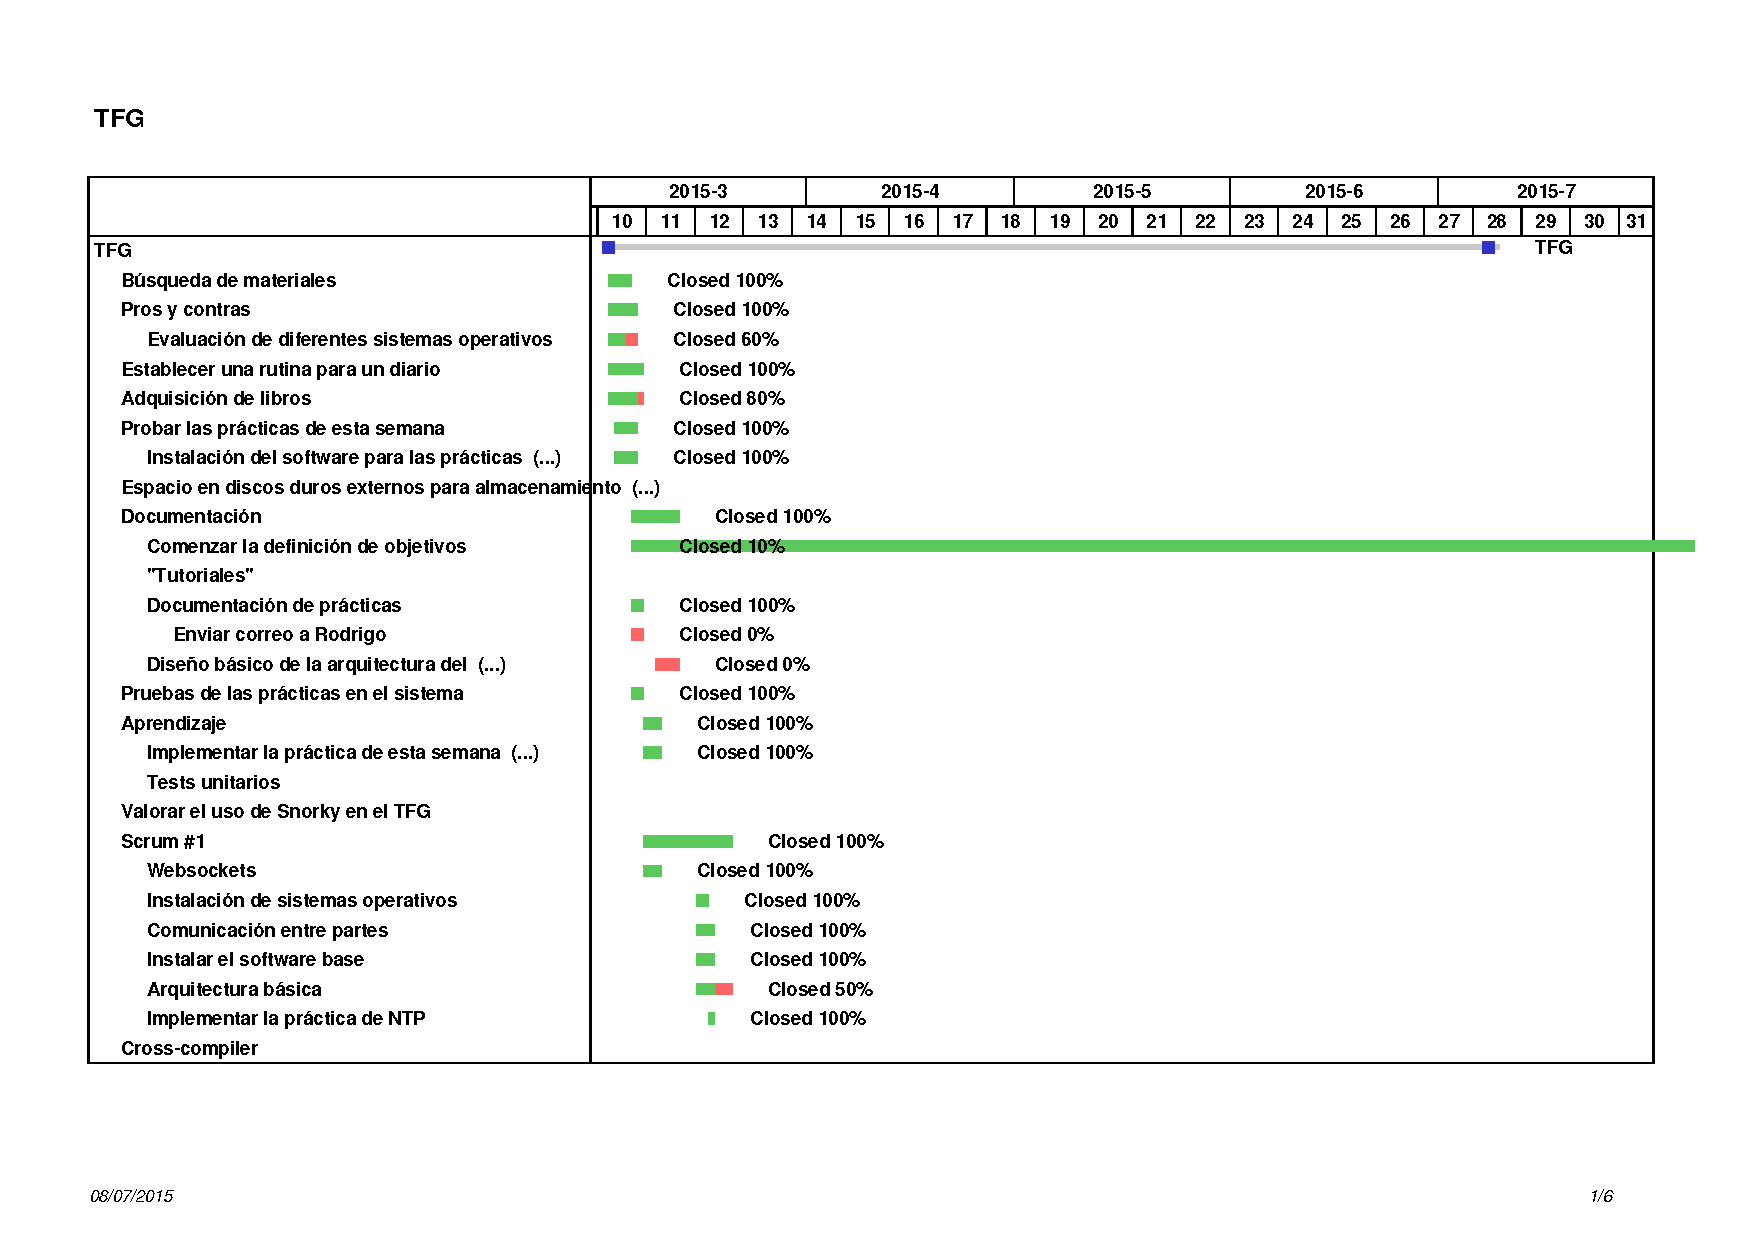
\includepdf[pages=-,pagecommand=\stepcounter{contador}\subsection{Diagrama de Gannt (parte \thecontador{})}]{./tfggantt.pdf}

\section{Gestión de la calidad}

La gestión de la calidad del código se realiza mediante la combinación de las siguientes estrategias:

\begin{itemize}
\item \textbf{Pruebas automatizadas}: Utilizando herramientas como unittest\footnote{\href{https://docs.python.org/2/library/unittest.html}{https://docs.python.org/2/library/unittest.html}} o Trial\footnote{\href{http://twistedmatrix.com/trac/wiki/TwistedTrial}{http://twistedmatrix.com/trac/wiki/TwistedTrial}} se ha realizado un desarrollo dirigido por pruebas.
\item \textbf{Pruebas manuales}: De forma similar a las pruebas automatizadas varios paquetes \textit{software} han sido creados utilizando pruebas manuales.
\item \textbf{Evaluaciones de usuario}: En aquellos casos en los que el \textit{software} creado deba ser utilizado de forma directa por un usuario humano se evaluará esta interacción mediante procedimientos de evaluación.
\item \textbf{Seguimiento de guías de estilo de código y utilización de herramientas de verificación}: Guías como la PEP 0008\footnote{\textit{Python Enhancement Proposal} 0008: \href{https://www.python.org/dev/peps/pep-0008/}{https://www.python.org/dev/peps/pep-0008/}} o \textbf{Pylint}\footnote{\href{http://www.pylint.org/}{http://www.pylint.org/}} asisten al desarrollador a la hora de crear código fuente que siga las convenciones propias de cada lenguaje. El uso de las mismas permite que el código sea más fácil de comprender por otros desarrolladores. \textbf{2to3}\footnote{\href{https://docs.python.org/2/library/2to3.html}{https://docs.python.org/2/library/2to3.html}} y \textbf{3to2}\footnote{\href{https://pypi.python.org/pypi/3to2/1.1.1}{https://pypi.python.org/pypi/3to2/1.1.1}}, entre otras utilidades, verifican la compatibilidad de código Python entre versiones. La guía de portabilidad de Python\footnote{\href{https://docs.python.org/3/howto/pyporting.html}{https://docs.python.org/3/howto/pyporting.html}} ha sido de gran utilidad en esta tarea.
\end{itemize}

\section{Comunicación}

La comunicación entre los diferentes integrantes del equipo se basa en reuniones presenciales entre todos los miembros. No ha sido necesaria una mayor formalización debido al reducido tamaño del equipo.


\section{Análisis de riesgos}

Uno de los mayores riesgos que las características del proyecto define es el incumplimiento de las estrictas fechas de desarrollo. Emplear demasiados recursos y tiempo en una tarea que no satisfaga los requisitos marcados inicialmente dañaría severamente el proyecto. Sin embargo, debido a la gran adaptabilidad que la metodología utilizada aporta ha sido posible determinar de forma temprana los problemas de una propuesta de solución.

\section{Control de versiones}

Es importante mantener un control de las diferentes versiones en desarrollo y productos creados durante el proceso de desarrollo. Dicho control facilita la gestión del proyecto, permite retornar el proyecto a un estado anterior o mantener de forma concurrente varias ramas de desarrollo.

Dado que el proyecto implica la construcción de un conjunto de herramientas que compongan un sistema, se utilizará un repositorio de código para cada una de ellas. El gestor elegido es \textbf{git}\footnote{\href{http://git-scm.com/}{http://git-scm.com/}}, debido a su carácter distribuido, posibilidad de trabajar con varias ramas de desarrollo y experiencia previa. Todo el código se almacena en el proveedor de alojamiento \textbf{Bitbucket}\footnote{\href{https://bitbucket.org/}{https://bitbucket.org/}}, actuando como copia de seguridad de los datos recogidos en el equipo local. 

Todos los repositorios son públicos, y están disponibles en el DVD adjunto a la documentación física y en la url \href{https://bitbucket.org/Alternhuman}{https://bitbucket.org/Alternhuman}.

Como conclusión cabe valorar el éxito de la metodología utilizada que ha facilitado, si no posibilitado, el buen devenir de este proyecto.

\end{document}